\documentclass[twoside]{book}

% Packages required by doxygen
\usepackage{fixltx2e}
\usepackage{calc}
\usepackage{doxygen}
\usepackage[export]{adjustbox} % also loads graphicx
\usepackage{graphicx}
\usepackage[utf8]{inputenc}
\usepackage{makeidx}
\usepackage{multicol}
\usepackage{multirow}
\PassOptionsToPackage{warn}{textcomp}
\usepackage{textcomp}
\usepackage[nointegrals]{wasysym}
\usepackage[table]{xcolor}

% Font selection
\usepackage[T1]{fontenc}
\usepackage[scaled=.90]{helvet}
\usepackage{courier}
\usepackage{amssymb}
\usepackage{sectsty}
\renewcommand{\familydefault}{\sfdefault}
\allsectionsfont{%
  \fontseries{bc}\selectfont%
  \color{darkgray}%
}
\renewcommand{\DoxyLabelFont}{%
  \fontseries{bc}\selectfont%
  \color{darkgray}%
}
\newcommand{\+}{\discretionary{\mbox{\scriptsize$\hookleftarrow$}}{}{}}

% Page & text layout
\usepackage{geometry}
\geometry{%
  a4paper,%
  top=2.5cm,%
  bottom=2.5cm,%
  left=2.5cm,%
  right=2.5cm%
}
\tolerance=750
\hfuzz=15pt
\hbadness=750
\setlength{\emergencystretch}{15pt}
\setlength{\parindent}{0cm}
\setlength{\parskip}{3ex plus 2ex minus 2ex}
\makeatletter
\renewcommand{\paragraph}{%
  \@startsection{paragraph}{4}{0ex}{-1.0ex}{1.0ex}{%
    \normalfont\normalsize\bfseries\SS@parafont%
  }%
}
\renewcommand{\subparagraph}{%
  \@startsection{subparagraph}{5}{0ex}{-1.0ex}{1.0ex}{%
    \normalfont\normalsize\bfseries\SS@subparafont%
  }%
}
\makeatother

% Headers & footers
\usepackage{fancyhdr}
\pagestyle{fancyplain}
\fancyhead[LE]{\fancyplain{}{\bfseries\thepage}}
\fancyhead[CE]{\fancyplain{}{}}
\fancyhead[RE]{\fancyplain{}{\bfseries\leftmark}}
\fancyhead[LO]{\fancyplain{}{\bfseries\rightmark}}
\fancyhead[CO]{\fancyplain{}{}}
\fancyhead[RO]{\fancyplain{}{\bfseries\thepage}}
\fancyfoot[LE]{\fancyplain{}{}}
\fancyfoot[CE]{\fancyplain{}{}}
\fancyfoot[RE]{\fancyplain{}{\bfseries\scriptsize Generated by Doxygen }}
\fancyfoot[LO]{\fancyplain{}{\bfseries\scriptsize Generated by Doxygen }}
\fancyfoot[CO]{\fancyplain{}{}}
\fancyfoot[RO]{\fancyplain{}{}}
\renewcommand{\footrulewidth}{0.4pt}
\renewcommand{\chaptermark}[1]{%
  \markboth{#1}{}%
}
\renewcommand{\sectionmark}[1]{%
  \markright{\thesection\ #1}%
}

% Indices & bibliography
\usepackage{natbib}
\usepackage[titles]{tocloft}
\setcounter{tocdepth}{3}
\setcounter{secnumdepth}{5}
\makeindex

% Hyperlinks (required, but should be loaded last)
\usepackage{ifpdf}
\ifpdf
  \usepackage[pdftex,pagebackref=true]{hyperref}
\else
  \usepackage[ps2pdf,pagebackref=true]{hyperref}
\fi
\hypersetup{%
  colorlinks=true,%
  linkcolor=blue,%
  citecolor=blue,%
  unicode%
}

% Custom commands
\newcommand{\clearemptydoublepage}{%
  \newpage{\pagestyle{empty}\cleardoublepage}%
}

\usepackage{caption}
\captionsetup{labelsep=space,justification=centering,font={bf},singlelinecheck=off,skip=4pt,position=top}

%===== C O N T E N T S =====

\begin{document}

% Titlepage & ToC
\hypersetup{pageanchor=false,
             bookmarksnumbered=true,
             pdfencoding=unicode
            }
\pagenumbering{roman}
\begin{titlepage}
\vspace*{7cm}
\begin{center}%
{\Large Asservissement }\\
\vspace*{1cm}
{\large Generated by Doxygen 1.8.11}\\
\end{center}
\end{titlepage}
\clearemptydoublepage
\tableofcontents
\clearemptydoublepage
\pagenumbering{arabic}
\hypersetup{pageanchor=true}

%--- Begin generated contents ---
\chapter{Class Index}
\section{Class List}
Here are the classes, structs, unions and interfaces with brief descriptions\+:\begin{DoxyCompactList}
\item\contentsline{section}{\hyperlink{class_asservissement}{Asservissement} }{\pageref{class_asservissement}}{}
\item\contentsline{section}{\hyperlink{class_moteur}{Moteur} }{\pageref{class_moteur}}{}
\item\contentsline{section}{\hyperlink{class_odometrie}{Odometrie} }{\pageref{class_odometrie}}{}
\item\contentsline{section}{\hyperlink{class_p_i_d}{P\+ID} }{\pageref{class_p_i_d}}{}
\item\contentsline{section}{\hyperlink{struct_pid_coeff}{Pid\+Coeff} }{\pageref{struct_pid_coeff}}{}
\item\contentsline{section}{\hyperlink{struct_position}{Position} }{\pageref{struct_position}}{}
\item\contentsline{section}{\hyperlink{struct_tick}{Tick} }{\pageref{struct_tick}}{}
\item\contentsline{section}{\hyperlink{struct_vitesse}{Vitesse} }{\pageref{struct_vitesse}}{}
\end{DoxyCompactList}

\chapter{File Index}
\section{File List}
Here is a list of all documented files with brief descriptions\+:\begin{DoxyCompactList}
\item\contentsline{section}{\hyperlink{asservissement_8cpp}{asservissement.\+cpp} \\*Classe \hyperlink{class_asservissement}{Asservissement}. Code asservissement du grand Robot, permet d\textquotesingle{}asservir en angle et en position le robot pour envoyer une consigne vitesse au robot à l\textquotesingle{}aide d\textquotesingle{}un \hyperlink{class_p_i_d}{P\+ID} Il y a des define a mettre a jour }{\pageref{asservissement_8cpp}}{}
\item\contentsline{section}{\hyperlink{asservissement_8h}{asservissement.\+h} \\*Entête classe asservissement du grand robot }{\pageref{asservissement_8h}}{}
\item\contentsline{section}{\hyperlink{moteur_8cpp}{moteur.\+cpp} \\*Code contrôle des moteurs du grand Robot. Ce programme permet d\textquotesingle{}initialiser et d\textquotesingle{}envoyer 4 P\+WM (2 P\+WM pour chaque moteur) au driver moteur }{\pageref{moteur_8cpp}}{}
\item\contentsline{section}{\hyperlink{moteur_8h}{moteur.\+h} \\*Classe moteur du grand robot }{\pageref{moteur_8h}}{}
\item\contentsline{section}{\hyperlink{odometrie_8cpp}{odometrie.\+cpp} \\*Code odometrie du grand robot. Permet de connaitre la prosition du robot sur l\textquotesingle{}axe x,y ainsi que son angle }{\pageref{odometrie_8cpp}}{}
\item\contentsline{section}{\hyperlink{odometrie_8h}{odometrie.\+h} \\*Classe odometrie du grand robot }{\pageref{odometrie_8h}}{}
\item\contentsline{section}{\hyperlink{_p_i_d_8cpp}{P\+I\+D.\+cpp} \\*Code Proportionnel Intégrateur Dérivateur (\hyperlink{class_p_i_d}{P\+ID}) du grand Robot. Permet de corriger la consigne de sortie en fonction de la consigne d\textquotesingle{}entrée (éviter les oscilations de position et d\textquotesingle{}angle) }{\pageref{_p_i_d_8cpp}}{}
\item\contentsline{section}{\hyperlink{_p_i_d_8h}{P\+I\+D.\+h} \\*Class \hyperlink{class_p_i_d}{P\+ID} Proportionnel Intégrateur Dérivateur du grand robot }{\pageref{_p_i_d_8h}}{}
\item\contentsline{section}{{\bfseries structures.\+h} }{\pageref{structures_8h}}{}
\end{DoxyCompactList}

\chapter{Class Documentation}
\hypertarget{class_asservissement}{}\section{Asservissement Class Reference}
\label{class_asservissement}\index{Asservissement@{Asservissement}}
\subsection*{Public Member Functions}
\begin{DoxyCompactItemize}
\item 
{\bfseries Asservissement} (double periode, \hyperlink{class_moteur}{Moteur} grobot)\hypertarget{class_asservissement_a602ab222a93b691ada69cfe11208faf2}{}\label{class_asservissement_a602ab222a93b691ada69cfe11208faf2}

\item 
double {\bfseries bound\+Error} (double e)\hypertarget{class_asservissement_af459078c269e8872c8f9585774b5aee1}{}\label{class_asservissement_af459078c269e8872c8f9585774b5aee1}

\item 
double {\bfseries cont\+Distance} (\hyperlink{struct_position}{Position} destination, \hyperlink{struct_position}{Position} robot)\hypertarget{class_asservissement_a46c56c095e7a01174809cf2683782113}{}\label{class_asservissement_a46c56c095e7a01174809cf2683782113}

\item 
double {\bfseries cont\+Angle} (\hyperlink{struct_position}{Position} destination, \hyperlink{struct_position}{Position} robot)\hypertarget{class_asservissement_a94e0a6d4d378d41daa14bce3f07ea422}{}\label{class_asservissement_a94e0a6d4d378d41daa14bce3f07ea422}

\item 
void {\bfseries new\+Order\+Angle} (\hyperlink{struct_position}{Position} destination, double theta\+\_\+order)\hypertarget{class_asservissement_ab025d475e1daec59e2656fa505ce726d}{}\label{class_asservissement_ab025d475e1daec59e2656fa505ce726d}

\item 
void {\bfseries check\+Enslavement\+Type} (double error\+\_\+L, double error\+\_\+T, int $\ast$asserv\+\_\+L, int $\ast$asserv\+\_\+T)\hypertarget{class_asservissement_a2accd4d87bcaded977d64923388f1a5a}{}\label{class_asservissement_a2accd4d87bcaded977d64923388f1a5a}

\item 
void {\bfseries add\+P\+WM} (double pwm\+Control\+\_\+L, double pwm\+Control\+\_\+T, int sens)\hypertarget{class_asservissement_ad922a1864e6075436f211bd94e019dee}{}\label{class_asservissement_ad922a1864e6075436f211bd94e019dee}

\item 
void {\bfseries appliquer\+Ordre} (\hyperlink{struct_position}{Position} destination, \hyperlink{struct_position}{Position} robot, int sens)\hypertarget{class_asservissement_a8eeb4d2ea61bdad69173765ef3dc05b4}{}\label{class_asservissement_a8eeb4d2ea61bdad69173765ef3dc05b4}

\item 
void {\bfseries atteindre\+Angle} (\hyperlink{struct_position}{Position} destination, \hyperlink{struct_position}{Position} robot)\hypertarget{class_asservissement_a31365ebbbf9f9309d9b4556e4e753dff}{}\label{class_asservissement_a31365ebbbf9f9309d9b4556e4e753dff}

\item 
void {\bfseries atteindre\+Distance} (\hyperlink{struct_position}{Position} destination, \hyperlink{struct_position}{Position} robot)\hypertarget{class_asservissement_afe6baa10d9ec255aa5268122f0c9b6d5}{}\label{class_asservissement_afe6baa10d9ec255aa5268122f0c9b6d5}

\item 
void {\bfseries curve} (\hyperlink{struct_position}{Position} destination, \hyperlink{struct_position}{Position} robot)\hypertarget{class_asservissement_a0017ded3b839ece7403a5c63a2f50fe8}{}\label{class_asservissement_a0017ded3b839ece7403a5c63a2f50fe8}

\item 
void {\bfseries atteindre\+Position} (\hyperlink{struct_position}{Position} destination, \hyperlink{struct_position}{Position} robot)\hypertarget{class_asservissement_a0ddbc9243384337c1f3af07ffc8b85b0}{}\label{class_asservissement_a0ddbc9243384337c1f3af07ffc8b85b0}

\item 
double {\bfseries abs1} (double nombre)\hypertarget{class_asservissement_a7f53388f95bfd3450d4da5a1c0a45075}{}\label{class_asservissement_a7f53388f95bfd3450d4da5a1c0a45075}

\end{DoxyCompactItemize}


The documentation for this class was generated from the following files\+:\begin{DoxyCompactItemize}
\item 
\hyperlink{asservissement_8h}{asservissement.\+h}\item 
\hyperlink{asservissement_8cpp}{asservissement.\+cpp}\end{DoxyCompactItemize}

\hypertarget{class_moteur}{}\section{Moteur Class Reference}
\label{class_moteur}\index{Moteur@{Moteur}}
\subsection*{Public Member Functions}
\begin{DoxyCompactItemize}
\item 
void {\bfseries init\+P\+WM} ()\hypertarget{class_moteur_a89e10e5be14072650f37037ffd912fd0}{}\label{class_moteur_a89e10e5be14072650f37037ffd912fd0}

\item 
int {\bfseries convertir\+\_\+pourcentage\+\_\+en\+\_\+octet} ()\hypertarget{class_moteur_a455ceec5ff8d7d51f8a823259762131c}{}\label{class_moteur_a455ceec5ff8d7d51f8a823259762131c}

\item 
void {\bfseries brake} (int choix\+\_\+moteur)\hypertarget{class_moteur_a94ce68461266cf4cf7fa85ed004454e0}{}\label{class_moteur_a94ce68461266cf4cf7fa85ed004454e0}

\item 
void {\bfseries fonctionnement\+\_\+moteur} (double vitesse\+Gauche, double vitesse\+Droit)\hypertarget{class_moteur_aa637ddd3e6ad5878e39d251db62b6862}{}\label{class_moteur_aa637ddd3e6ad5878e39d251db62b6862}

\end{DoxyCompactItemize}


The documentation for this class was generated from the following files\+:\begin{DoxyCompactItemize}
\item 
\hyperlink{moteur_8h}{moteur.\+h}\item 
\hyperlink{moteur_8cpp}{moteur.\+cpp}\end{DoxyCompactItemize}

\hypertarget{class_odometrie}{}\section{Odometrie Class Reference}
\label{class_odometrie}\index{Odometrie@{Odometrie}}
\subsection*{Public Member Functions}
\begin{DoxyCompactItemize}
\item 
void {\bfseries calculer\+\_\+pas} ()\hypertarget{class_odometrie_ae68ca6d28bf47ec2c1835714a9839456}{}\label{class_odometrie_ae68ca6d28bf47ec2c1835714a9839456}

\item 
void {\bfseries calculer\+\_\+variation\+\_\+distance} ()\hypertarget{class_odometrie_ab4689aa19bfc65ff5d0704d65ea41e0e}{}\label{class_odometrie_ab4689aa19bfc65ff5d0704d65ea41e0e}

\item 
void \hyperlink{class_odometrie_a6900512580f5347a37c4cb8b5fd93043}{calculer\+\_\+variation\+\_\+angle} ()
\item 
void {\bfseries calculer\+\_\+\+Impulion\+Parmm} ()\hypertarget{class_odometrie_a3777f956fc5f4d0e5087cc873b4c6147}{}\label{class_odometrie_a3777f956fc5f4d0e5087cc873b4c6147}

\item 
void {\bfseries calculer\+\_\+\+Impulsion\+Parrad} ()\hypertarget{class_odometrie_ac0661c3b98db0e45c096d11181ecb983}{}\label{class_odometrie_ac0661c3b98db0e45c096d11181ecb983}

\item 
void {\bfseries calculer\+\_\+distance\+Parcourue\+Roue} (\hyperlink{struct_tick}{Tick} codeuse)\hypertarget{class_odometrie_aa9f3987c74ae16c6bb73475f6fa995d5}{}\label{class_odometrie_aa9f3987c74ae16c6bb73475f6fa995d5}

\item 
void {\bfseries retourner\+Valeur} (\hyperlink{struct_position}{Position} $\ast$roue\+Codeuse, \hyperlink{struct_tick}{Tick} codeuse)\hypertarget{class_odometrie_a8b9266574fce4de4131421053e8fa73b}{}\label{class_odometrie_a8b9266574fce4de4131421053e8fa73b}

\item 
void {\bfseries calculer\+\_\+angle} (\hyperlink{struct_position}{Position} $\ast$destination, \hyperlink{struct_position}{Position} robot)\hypertarget{class_odometrie_a45bd260006f6f5e4596814c80c578025}{}\label{class_odometrie_a45bd260006f6f5e4596814c80c578025}

\item 
double {\bfseries calculer\+\_\+distance} (\hyperlink{struct_position}{Position} destination, \hyperlink{struct_position}{Position} robot)\hypertarget{class_odometrie_a49c4d594d1280d18302ad3274a732118}{}\label{class_odometrie_a49c4d594d1280d18302ad3274a732118}

\end{DoxyCompactItemize}


\subsection{Member Function Documentation}
\index{Odometrie@{Odometrie}!calculer\+\_\+variation\+\_\+angle@{calculer\+\_\+variation\+\_\+angle}}
\index{calculer\+\_\+variation\+\_\+angle@{calculer\+\_\+variation\+\_\+angle}!Odometrie@{Odometrie}}
\subsubsection[{\texorpdfstring{calculer\+\_\+variation\+\_\+angle()}{calculer_variation_angle()}}]{\setlength{\rightskip}{0pt plus 5cm}void Odometrie\+::calculer\+\_\+variation\+\_\+angle (
\begin{DoxyParamCaption}
{}
\end{DoxyParamCaption}
)}\hypertarget{class_odometrie_a6900512580f5347a37c4cb8b5fd93043}{}\label{class_odometrie_a6900512580f5347a37c4cb8b5fd93043}
m\+\_\+distance\+\_\+roue\+\_\+codeuse; 

The documentation for this class was generated from the following files\+:\begin{DoxyCompactItemize}
\item 
\hyperlink{odometrie_8h}{odometrie.\+h}\item 
\hyperlink{odometrie_8cpp}{odometrie.\+cpp}\end{DoxyCompactItemize}

\hypertarget{class_p_i_d}{}\section{P\+ID Class Reference}
\label{class_p_i_d}\index{P\+ID@{P\+ID}}
\subsection*{Public Member Functions}
\begin{DoxyCompactItemize}
\item 
{\bfseries P\+ID} (double kP, double kI, double kD, double periode)\hypertarget{class_p_i_d_ad10969b52a5c2c78775fee51de5a595c}{}\label{class_p_i_d_ad10969b52a5c2c78775fee51de5a595c}

\item 
void {\bfseries reset\+P\+ID} (double error)\hypertarget{class_p_i_d_a3fcf72ad59b79e2a5a67b6d110c37b3f}{}\label{class_p_i_d_a3fcf72ad59b79e2a5a67b6d110c37b3f}

\item 
double {\bfseries compute\+P\+ID} (double error)\hypertarget{class_p_i_d_a9777e338d838fbafc098dc15a28d6d1f}{}\label{class_p_i_d_a9777e338d838fbafc098dc15a28d6d1f}

\end{DoxyCompactItemize}


The documentation for this class was generated from the following files\+:\begin{DoxyCompactItemize}
\item 
\hyperlink{_p_i_d_8h}{P\+I\+D.\+h}\item 
\hyperlink{_p_i_d_8cpp}{P\+I\+D.\+cpp}\end{DoxyCompactItemize}

\hypertarget{struct_pid_coeff}{}\section{Pid\+Coeff Struct Reference}
\label{struct_pid_coeff}\index{Pid\+Coeff@{Pid\+Coeff}}
\subsection*{Public Attributes}
\begin{DoxyCompactItemize}
\item 
double {\bfseries kP}\hypertarget{struct_pid_coeff_ac197194a5709f444836560eb26c72529}{}\label{struct_pid_coeff_ac197194a5709f444836560eb26c72529}

\item 
double {\bfseries kI}\hypertarget{struct_pid_coeff_ab0fbc32f5a94c8656d0bf8b22361d175}{}\label{struct_pid_coeff_ab0fbc32f5a94c8656d0bf8b22361d175}

\item 
double {\bfseries kD}\hypertarget{struct_pid_coeff_a26142a9100b6d62fd007712190113939}{}\label{struct_pid_coeff_a26142a9100b6d62fd007712190113939}

\end{DoxyCompactItemize}


The documentation for this struct was generated from the following file\+:\begin{DoxyCompactItemize}
\item 
structures.\+h\end{DoxyCompactItemize}

\hypertarget{struct_position}{}\section{Position Struct Reference}
\label{struct_position}\index{Position@{Position}}
\subsection*{Public Attributes}
\begin{DoxyCompactItemize}
\item 
double {\bfseries x}\hypertarget{struct_position_a9abbe738bad177de91fe4774099c1260}{}\label{struct_position_a9abbe738bad177de91fe4774099c1260}

\item 
double {\bfseries y}\hypertarget{struct_position_a75f48c2a1d2c7131b8be1a0687ae72c8}{}\label{struct_position_a75f48c2a1d2c7131b8be1a0687ae72c8}

\item 
double {\bfseries thetha}\hypertarget{struct_position_a575782e58b84c940b73b4b13d79bc90b}{}\label{struct_position_a575782e58b84c940b73b4b13d79bc90b}

\item 
double {\bfseries distance}\hypertarget{struct_position_a5f42dba8245012ff325521a88ff7a892}{}\label{struct_position_a5f42dba8245012ff325521a88ff7a892}

\end{DoxyCompactItemize}


The documentation for this struct was generated from the following file\+:\begin{DoxyCompactItemize}
\item 
structures.\+h\end{DoxyCompactItemize}

\hypertarget{struct_tick}{}\section{Tick Struct Reference}
\label{struct_tick}\index{Tick@{Tick}}
\subsection*{Public Attributes}
\begin{DoxyCompactItemize}
\item 
long int {\bfseries ND}\hypertarget{struct_tick_a788ee9eb9f9b0d6f234cb86f8fa100dd}{}\label{struct_tick_a788ee9eb9f9b0d6f234cb86f8fa100dd}

\item 
long int {\bfseries NG}\hypertarget{struct_tick_a60a0aa37b32f1f280febe76bd67081bf}{}\label{struct_tick_a60a0aa37b32f1f280febe76bd67081bf}

\end{DoxyCompactItemize}


The documentation for this struct was generated from the following file\+:\begin{DoxyCompactItemize}
\item 
structures.\+h\end{DoxyCompactItemize}

\hypertarget{struct_vitesse}{}\section{Vitesse Struct Reference}
\label{struct_vitesse}\index{Vitesse@{Vitesse}}
\subsection*{Public Attributes}
\begin{DoxyCompactItemize}
\item 
double {\bfseries motorG}\hypertarget{struct_vitesse_a98d077010cc73824784e494b23de1459}{}\label{struct_vitesse_a98d077010cc73824784e494b23de1459}

\item 
double {\bfseries motorD}\hypertarget{struct_vitesse_a8d32cbd41e826948a853243fe713a20b}{}\label{struct_vitesse_a8d32cbd41e826948a853243fe713a20b}

\end{DoxyCompactItemize}


The documentation for this struct was generated from the following file\+:\begin{DoxyCompactItemize}
\item 
structures.\+h\end{DoxyCompactItemize}

\chapter{File Documentation}
\hypertarget{asservissement_8cpp}{}\section{asservissement.\+cpp File Reference}
\label{asservissement_8cpp}\index{asservissement.\+cpp@{asservissement.\+cpp}}


Classe \hyperlink{class_asservissement}{Asservissement}. Code asservissement du grand Robot, permet d\textquotesingle{}asservir en angle et en position le robot pour envoyer une consigne vitesse au robot à l\textquotesingle{}aide d\textquotesingle{}un \hyperlink{class_p_i_d}{P\+ID} Il y a des define a mettre a jour.  


{\ttfamily \#include \char`\"{}asservissement.\+h\char`\"{}}\\*
{\ttfamily \#include \char`\"{}math.\+h\char`\"{}}\\*
{\ttfamily \#include \char`\"{}structures.\+h\char`\"{}}\\*
{\ttfamily \#include \char`\"{}odometrie.\+h\char`\"{}}\\*
{\ttfamily \#include \char`\"{}moteur.\+h\char`\"{}}\\*
{\ttfamily \#include \char`\"{}P\+I\+D.\+h\char`\"{}}\\*
{\ttfamily \#include \char`\"{}Arduino.\+h\char`\"{}}\\*
Include dependency graph for asservissement.\+cpp\+:
\nopagebreak
\begin{figure}[H]
\begin{center}
\leavevmode
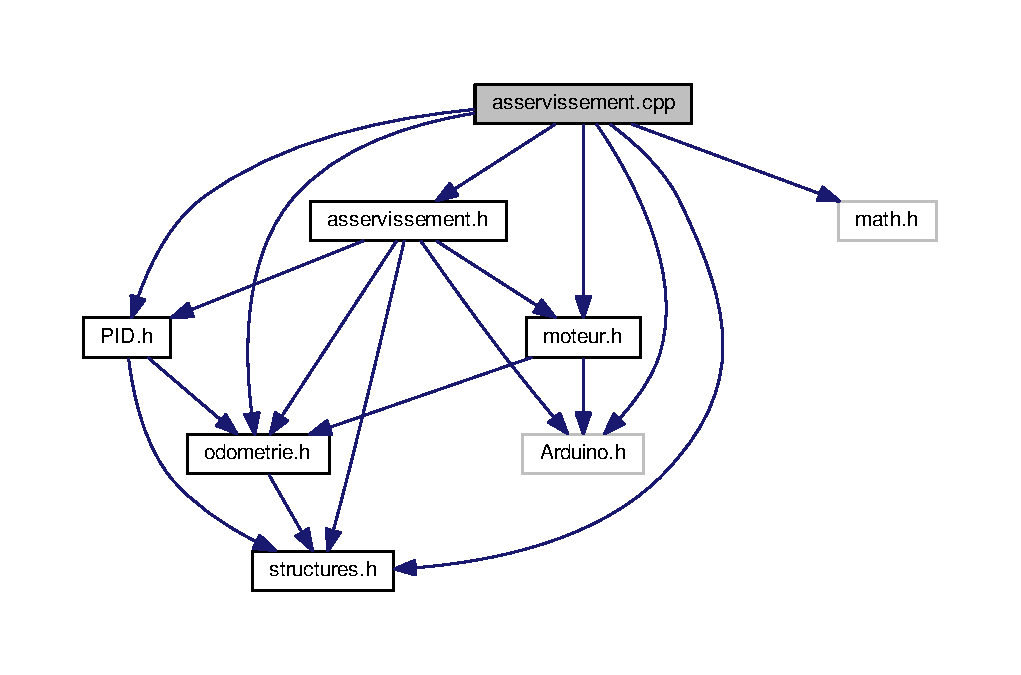
\includegraphics[width=350pt]{asservissement_8cpp__incl}
\end{center}
\end{figure}
\subsection*{Macros}
\begin{DoxyCompactItemize}
\item 
\#define {\bfseries PI}~3.\+14159\hypertarget{asservissement_8cpp_a598a3330b3c21701223ee0ca14316eca}{}\label{asservissement_8cpp_a598a3330b3c21701223ee0ca14316eca}

\end{DoxyCompactItemize}


\subsection{Detailed Description}
Classe \hyperlink{class_asservissement}{Asservissement}. Code asservissement du grand Robot, permet d\textquotesingle{}asservir en angle et en position le robot pour envoyer une consigne vitesse au robot à l\textquotesingle{}aide d\textquotesingle{}un \hyperlink{class_p_i_d}{P\+ID} Il y a des define a mettre a jour. 

Codé pour \char`\"{}\+Spark core\char`\"{} www.\+spark.\+io

Par \+: Thibaut L\+O\+C\+Q\+U\+ET Janvier 2013 Modification\+: Clément L\+E\+T\+E\+L\+L\+I\+ER Mars 2014 Modification\+: Nicolas S\+O\+B\+C\+Z\+AK Octobre 2016 
\hypertarget{asservissement_8h}{}\section{asservissement.\+h File Reference}
\label{asservissement_8h}\index{asservissement.\+h@{asservissement.\+h}}


entête classe asservissement du grand robot  


{\ttfamily \#include \char`\"{}structures.\+h\char`\"{}}\\*
{\ttfamily \#include \char`\"{}odometrie.\+h\char`\"{}}\\*
{\ttfamily \#include \char`\"{}moteur.\+h\char`\"{}}\\*
{\ttfamily \#include \char`\"{}P\+I\+D.\+h\char`\"{}}\\*
{\ttfamily \#include \char`\"{}Arduino.\+h\char`\"{}}\\*
Include dependency graph for asservissement.\+h\+:
\nopagebreak
\begin{figure}[H]
\begin{center}
\leavevmode
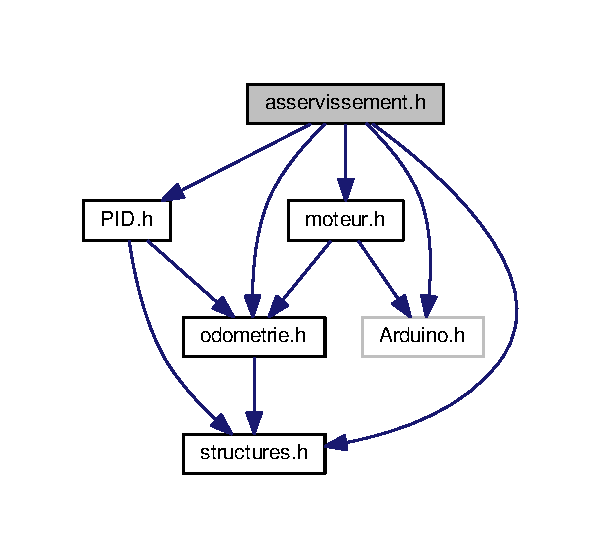
\includegraphics[width=289pt]{asservissement_8h__incl}
\end{center}
\end{figure}
This graph shows which files directly or indirectly include this file\+:
\nopagebreak
\begin{figure}[H]
\begin{center}
\leavevmode
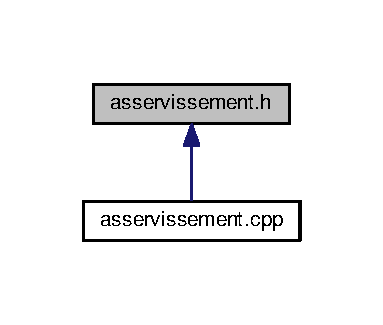
\includegraphics[width=184pt]{asservissement_8h__dep__incl}
\end{center}
\end{figure}
\subsection*{Classes}
\begin{DoxyCompactItemize}
\item 
class \hyperlink{class_asservissement}{Asservissement}
\end{DoxyCompactItemize}
\subsection*{Macros}
\begin{DoxyCompactItemize}
\item 
\#define {\bfseries E\+R\+R\+O\+R\+\_\+\+L\+\_\+\+A\+C\+C\+E\+P\+T\+ED}~10.\+0\hypertarget{asservissement_8h_aec7c82e3146dcb6ce0d1570861a1aaed}{}\label{asservissement_8h_aec7c82e3146dcb6ce0d1570861a1aaed}

\item 
\#define {\bfseries E\+R\+R\+O\+R\+\_\+\+T\+H\+E\+T\+A\+\_\+\+A\+C\+C\+E\+P\+T\+ED}~1.\+0\hypertarget{asservissement_8h_a9c421b2f916d0543806c67699b51ae23}{}\label{asservissement_8h_a9c421b2f916d0543806c67699b51ae23}

\end{DoxyCompactItemize}


\subsection{Detailed Description}
entête classe asservissement du grand robot 

Codé pour \char`\"{}\+Spark core\char`\"{} www.\+spark.\+io

Par\+: Clément L\+E\+T\+E\+L\+L\+I\+ER Mars 2014 Modification\+: Nicolas S\+O\+B\+C\+Z\+AK Octobre 2016 
\hypertarget{moteur_8cpp}{}\section{moteur.\+cpp File Reference}
\label{moteur_8cpp}\index{moteur.\+cpp@{moteur.\+cpp}}


Code contrôle des moteurs du grand Robot. Ce programme permet d\textquotesingle{}initialiser et d\textquotesingle{}envoyer 4 P\+WM (2 P\+WM pour chaque moteur) au driver moteur.  


{\ttfamily \#include \char`\"{}odometrie.\+h\char`\"{}}\\*
{\ttfamily \#include \char`\"{}Arduino.\+h\char`\"{}}\\*
{\ttfamily \#include \char`\"{}moteur.\+h\char`\"{}}\\*
Include dependency graph for moteur.\+cpp\+:
\nopagebreak
\begin{figure}[H]
\begin{center}
\leavevmode
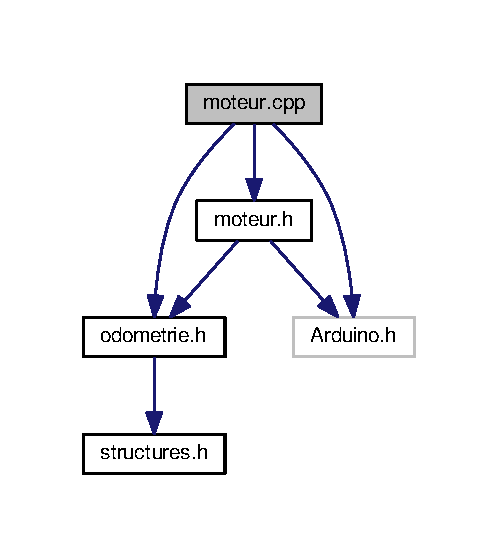
\includegraphics[width=239pt]{moteur_8cpp__incl}
\end{center}
\end{figure}
\subsection*{Macros}
\begin{DoxyCompactItemize}
\item 
\#define {\bfseries P\+W\+M\+\_\+\+F\+R\+EQ}~20000\hypertarget{moteur_8cpp_a76fe84d83b8d236bd4f0d20d7e2ed06f}{}\label{moteur_8cpp_a76fe84d83b8d236bd4f0d20d7e2ed06f}

\end{DoxyCompactItemize}
\subsection*{Variables}
\begin{DoxyCompactItemize}
\item 
uint16\+\_\+t {\bfseries T\+I\+M\+\_\+\+A\+RR} = (uint16\+\_\+t)(24000000 / P\+W\+M\+\_\+\+F\+R\+EQ) -\/ 1\hypertarget{moteur_8cpp_a5cf0310b8878ffe11e869ab580b8b3ab}{}\label{moteur_8cpp_a5cf0310b8878ffe11e869ab580b8b3ab}

\end{DoxyCompactItemize}


\subsection{Detailed Description}
Code contrôle des moteurs du grand Robot. Ce programme permet d\textquotesingle{}initialiser et d\textquotesingle{}envoyer 4 P\+WM (2 P\+WM pour chaque moteur) au driver moteur. 

Codé pour \char`\"{}\+Spark core\char`\"{} www.\+spark.\+io

Par \+: Clément L\+E\+T\+E\+L\+L\+I\+ER Mars 2014 Modification\+: Nicolas S\+O\+B\+C\+Z\+AK Octobre 2016 
\hypertarget{moteur_8h}{}\section{moteur.\+h File Reference}
\label{moteur_8h}\index{moteur.\+h@{moteur.\+h}}


Classe moteur du grand robot.  


{\ttfamily \#include \char`\"{}odometrie.\+h\char`\"{}}\\*
{\ttfamily \#include \char`\"{}Arduino.\+h\char`\"{}}\\*
Include dependency graph for moteur.\+h\+:
\nopagebreak
\begin{figure}[H]
\begin{center}
\leavevmode
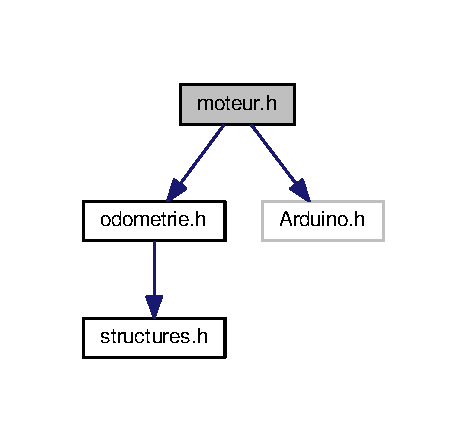
\includegraphics[width=224pt]{moteur_8h__incl}
\end{center}
\end{figure}
This graph shows which files directly or indirectly include this file\+:
\nopagebreak
\begin{figure}[H]
\begin{center}
\leavevmode
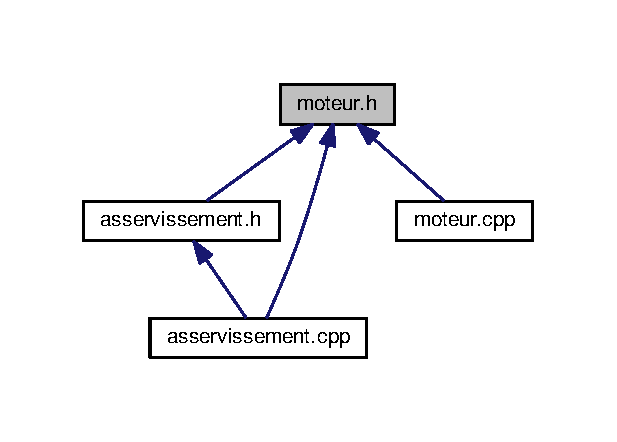
\includegraphics[width=296pt]{moteur_8h__dep__incl}
\end{center}
\end{figure}
\subsection*{Classes}
\begin{DoxyCompactItemize}
\item 
class \hyperlink{class_moteur}{Moteur}
\end{DoxyCompactItemize}
\subsection*{Macros}
\begin{DoxyCompactItemize}
\item 
\#define {\bfseries P\+M\+W\+\_\+\+M\+O\+T\+E\+U\+R\+\_\+\+A0}~5\hypertarget{moteur_8h_a50659f039de0d263938f621e0c8bc625}{}\label{moteur_8h_a50659f039de0d263938f621e0c8bc625}

\item 
\#define {\bfseries P\+M\+W\+\_\+\+M\+O\+T\+E\+U\+R\+\_\+\+A1}~4\hypertarget{moteur_8h_ac127249233a552dac7435631c046cd8e}{}\label{moteur_8h_ac127249233a552dac7435631c046cd8e}

\item 
\#define {\bfseries P\+M\+W\+\_\+\+M\+O\+T\+E\+U\+R\+\_\+\+B0}~7\hypertarget{moteur_8h_a137e3e39f06ac1effdd8d04523d25149}{}\label{moteur_8h_a137e3e39f06ac1effdd8d04523d25149}

\item 
\#define {\bfseries P\+M\+W\+\_\+\+M\+O\+T\+E\+U\+R\+\_\+\+B1}~6\hypertarget{moteur_8h_a59480bed1316437507c762cc756036ef}{}\label{moteur_8h_a59480bed1316437507c762cc756036ef}

\end{DoxyCompactItemize}


\subsection{Detailed Description}
Classe moteur du grand robot. 

Codé pour \char`\"{}\+Spark core\char`\"{} www.\+spark.\+io

Par\+: Clément L\+E\+T\+E\+L\+L\+I\+ER Mars 2014 Modification\+: Nicolas S\+O\+B\+C\+Z\+AK Octobre 2016 
\hypertarget{odometrie_8cpp}{}\section{odometrie.\+cpp File Reference}
\label{odometrie_8cpp}\index{odometrie.\+cpp@{odometrie.\+cpp}}


Code odometrie du grand robot. Permet de connaitre la prosition du robot sur l\textquotesingle{}axe x,y ainsi que son angle.  


{\ttfamily \#include \char`\"{}structures.\+h\char`\"{}}\\*
{\ttfamily \#include \char`\"{}odometrie.\+h\char`\"{}}\\*
{\ttfamily \#include \char`\"{}math.\+h\char`\"{}}\\*
Include dependency graph for odometrie.\+cpp\+:
\nopagebreak
\begin{figure}[H]
\begin{center}
\leavevmode
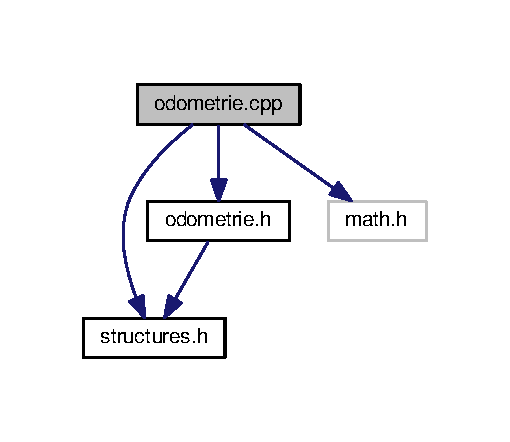
\includegraphics[width=245pt]{odometrie_8cpp__incl}
\end{center}
\end{figure}
\subsection*{Macros}
\begin{DoxyCompactItemize}
\item 
\#define {\bfseries PI}~3.\+14159\hypertarget{odometrie_8cpp_a598a3330b3c21701223ee0ca14316eca}{}\label{odometrie_8cpp_a598a3330b3c21701223ee0ca14316eca}

\end{DoxyCompactItemize}


\subsection{Detailed Description}
Code odometrie du grand robot. Permet de connaitre la prosition du robot sur l\textquotesingle{}axe x,y ainsi que son angle. 

Codé pour \char`\"{}\+Spark core\char`\"{} www.\+spark.\+io

Par\+: Clément L\+E\+T\+E\+L\+L\+I\+ER Mars 2014 Modification\+: Nicolas S\+O\+B\+C\+Z\+AK Octobre 2016 
\hypertarget{odometrie_8h}{}\section{odometrie.\+h File Reference}
\label{odometrie_8h}\index{odometrie.\+h@{odometrie.\+h}}


Classe odometrie du grand robot.  


{\ttfamily \#include \char`\"{}structures.\+h\char`\"{}}\\*
Include dependency graph for odometrie.\+h\+:
\nopagebreak
\begin{figure}[H]
\begin{center}
\leavevmode
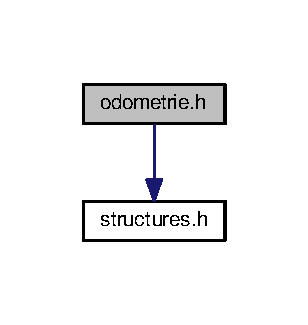
\includegraphics[width=148pt]{odometrie_8h__incl}
\end{center}
\end{figure}
This graph shows which files directly or indirectly include this file\+:
\nopagebreak
\begin{figure}[H]
\begin{center}
\leavevmode
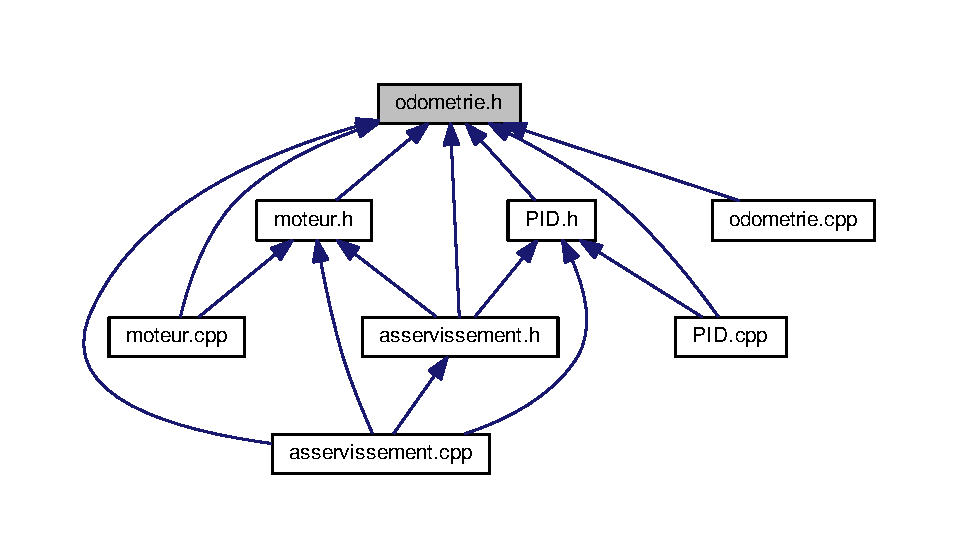
\includegraphics[width=350pt]{odometrie_8h__dep__incl}
\end{center}
\end{figure}
\subsection*{Classes}
\begin{DoxyCompactItemize}
\item 
class \hyperlink{class_odometrie}{Odometrie}
\end{DoxyCompactItemize}


\subsection{Detailed Description}
Classe odometrie du grand robot. 

Codé pour \char`\"{}\+Spark core\char`\"{} www.\+spark.\+io

Par\+: Clément L\+E\+T\+E\+L\+L\+I\+ER Mars 2014 Modification\+: Nicolas S\+O\+B\+C\+Z\+AK Octobre 2016 
\hypertarget{_p_i_d_8cpp}{}\section{P\+I\+D.\+cpp File Reference}
\label{_p_i_d_8cpp}\index{P\+I\+D.\+cpp@{P\+I\+D.\+cpp}}


Code Proportionnel Intégrateur Dérivateur (\hyperlink{class_p_i_d}{P\+ID}) du grand Robot. Permet de corriger la consigne de sortie en fonction de la consigne d\textquotesingle{}entrée (éviter les oscilations de position et d\textquotesingle{}angle)  


{\ttfamily \#include \char`\"{}structures.\+h\char`\"{}}\\*
{\ttfamily \#include \char`\"{}odometrie.\+h\char`\"{}}\\*
{\ttfamily \#include \char`\"{}P\+I\+D.\+h\char`\"{}}\\*
Include dependency graph for P\+I\+D.\+cpp\+:
\nopagebreak
\begin{figure}[H]
\begin{center}
\leavevmode
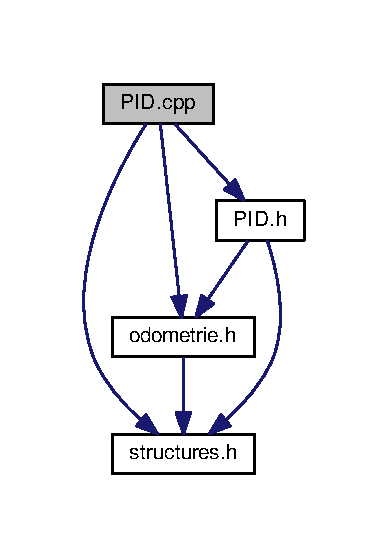
\includegraphics[width=186pt]{_p_i_d_8cpp__incl}
\end{center}
\end{figure}


\subsection{Detailed Description}
Code Proportionnel Intégrateur Dérivateur (\hyperlink{class_p_i_d}{P\+ID}) du grand Robot. Permet de corriger la consigne de sortie en fonction de la consigne d\textquotesingle{}entrée (éviter les oscilations de position et d\textquotesingle{}angle) 

Codé pour \char`\"{}\+Spark core\char`\"{} www.\+spark.\+io

Par \+: Thibaut L\+O\+C\+Q\+U\+ET Octobre 2012 Modification\+: Clément L\+E\+T\+E\+L\+L\+I\+ER Mars 2014 Modification\+: Nicolas S\+O\+B\+C\+Z\+AK Octobre 2016 
\hypertarget{_p_i_d_8h}{}\section{P\+I\+D.\+h File Reference}
\label{_p_i_d_8h}\index{P\+I\+D.\+h@{P\+I\+D.\+h}}


Class \hyperlink{class_p_i_d}{P\+ID} Proportionnel Intégrateur Dérivateur du grand robot.  


{\ttfamily \#include \char`\"{}structures.\+h\char`\"{}}\\*
{\ttfamily \#include \char`\"{}odometrie.\+h\char`\"{}}\\*
Include dependency graph for P\+I\+D.\+h\+:
\nopagebreak
\begin{figure}[H]
\begin{center}
\leavevmode
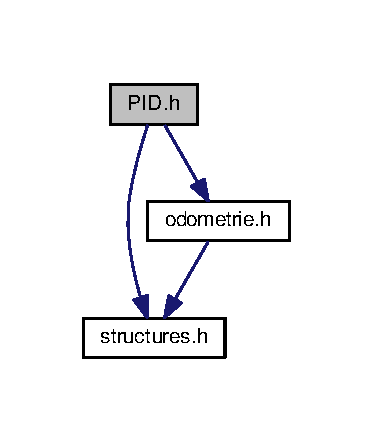
\includegraphics[width=179pt]{_p_i_d_8h__incl}
\end{center}
\end{figure}
This graph shows which files directly or indirectly include this file\+:
\nopagebreak
\begin{figure}[H]
\begin{center}
\leavevmode
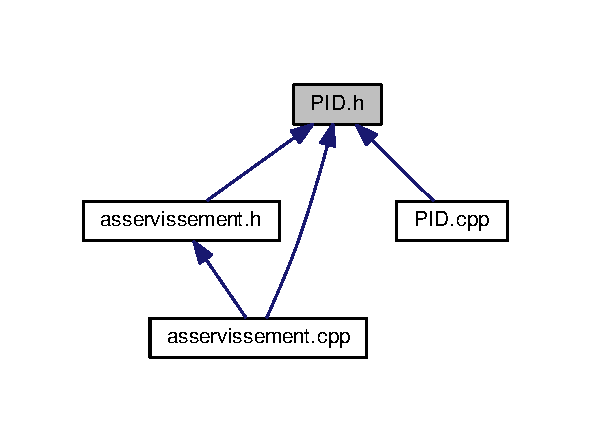
\includegraphics[width=284pt]{_p_i_d_8h__dep__incl}
\end{center}
\end{figure}
\subsection*{Classes}
\begin{DoxyCompactItemize}
\item 
class \hyperlink{class_p_i_d}{P\+ID}
\end{DoxyCompactItemize}


\subsection{Detailed Description}
Class \hyperlink{class_p_i_d}{P\+ID} Proportionnel Intégrateur Dérivateur du grand robot. 

Codé pour \char`\"{}\+Spark core\char`\"{} www.\+spark.\+io

Par\+: Clément L\+E\+T\+E\+L\+L\+I\+ER Mars 2014 Modification\+: Nicolas S\+O\+B\+C\+Z\+AK Octobre 2016 
%--- End generated contents ---

% Index
\backmatter
\newpage
\phantomsection
\clearemptydoublepage
\addcontentsline{toc}{chapter}{Index}
\printindex

\end{document}
